\section{VIX options and implied-volatility smiles}\label{sec:vix_options}

VIX futures are smooth concave functions of $\mathrm{VIX}_T^2$, so the static \RoughCertTilt{} bracket of
Theorem~\ref{thm:tilted} already attains sub-tick precision. VIX calls and puts introduce a payoff kink
at the strike $K$, degrading the single-tilt Lipschitz control \eqref{eq:tilted_opt_lip} from
$O(\varepsilon^4)$ to $O(\varepsilon^2)$. This section applies the 169-bit Arb \RoughCertCV{} engine of
Proposition~\ref{prop:arb}(c)--(e) to five published option and smile benchmarks, contrasting its precision
against \eqref{eq:tilted_opt_lip}, the order-three weak expansion of \citet{BourgeyDeMarcoGobet2023}, the
direct IV expansion of \citet{LiaoAgarwalBourgey2026}, the moment-matched lognormal proxy, and the multilevel
Monte Carlo benchmark of \citet{BourgeyDeMarco2022}. Every call, put, and Black-76 implied-volatility bracket
below carries the label \lab{Arb-certified} and propagates forward-price uncertainty rigorously via
Proposition~\ref{prop:arb}(e).

\subsection{Pure rough Bergomi: BDG Figure~6, LAB (2026), and stress smiles}\label{sec:pure_smiles}
We first audit the three-month VIX smile of \citet[Figure~6]{BourgeyDeMarcoGobet2023} ($H=0.10$,
$T=0.25$, $a=1.0$, $\Delta=1/12$, $\xi_0=0.235^2$) across nine log-moneyness strikes
$k=\log(K/F_{\mathrm{mid}})\in[-0.4,0.4]$ (Table~\ref{tab:vix_smiles}, top panel; Figure~\ref{fig:vix_smiles},
left). The comparisons use common physical strikes.
\begin{enumerate}
\item \emph{Conditional variance tightens the option control.} The static Lipschitz
  control \eqref{eq:tilted_opt_lip} gives a uniform option error bound of $\LipFigSix$ volatility points,
  whereas the Arb conditional-variance call brackets have widths $\FigSixCallWLo$--$\FigSixCallWHi$ volatility points
  (ratios of approximately $\LipRatioLo$--$\LipRatioHi$ against that bound), tightening smoothly into the out-of-the-money right wing.
\item \emph{Forward inflation induces systematic downward IV bias in BDG~(2023).} Although BDG's
  order-three call prices lie inside our Arb call brackets at six of nine strikes (falling outside by
  $+\SepKmFour$ at $k=-0.40$, $+\SepKmThree$ at $k=-0.30$, and $-\SepKpFour$ at $k=+0.40$), inverting those calls
  against BDG's own inflated order-three forward ($19.9367$ versus our Arb future $[19.9092,19.9152]$)
  shifts the BDG implied-volatility curve downward by $\FigSixIVGapLo$--$\FigSixIVGapHi$ percentage points
  below our Arb IV lower bound at \emph{all nine strikes} ($\BDGIVPureLo\%$--$\BDGIVPureHi\%$ versus $[113.48\%,114.05\%]$ to
  $[114.83\%,115.01\%]$).
\item \emph{Machine-verified positive VIX skew and lognormal failure.} Because the Arb IV upper bound at
  $k=-0.40$ ($114.05\%$) lies strictly below the Arb IV lower bound at $k=+0.40$ ($114.83\%$), the
  continuous rough-Bergomi VIX smile is machine-verified to be higher at the right endpoint by at least $\PureSkew$
  percentage points across $[-0.4,0.4]$. By contrast, the moment-matched lognormal proxy predicts a flat
  smile inside $[\LNIVPureLo\%,\LNIVPureHi\%]$, exceeding the Arb IV upper bound by
  $\LNAbovePureLo$--$\LNAbovePureHi$ percentage points at every strike.
\end{enumerate}

A flat-variance scaling check inspired by \citet{LiaoAgarwalBourgey2026} rescales the forward-variance
level ($\xi_0=0.24^2$, $H=0.10$, $a=1.0$, $T=0.25$, $\Delta=1/12$, seven strikes $k\in[-0.3,0.3]$). Flat scaling
of $\xi_0$ leaves Black-76 implied volatilities invariant ($[113.66\%,114.13\%]$ at $k=-0.30$ rising to
$[114.66\%,114.86\%]$ at $k=+0.30$, with all call widths $\ScaleCallWLo$--$\ScaleCallWHi$ volatility points and
forward $[20.3328,20.3390]$), while BDG order-three IV remains $\ScaleIVGapLo$--$\ScaleIVGapHi$ percentage points below the
Arb lower bound at every sampled strike.

Under the six-month stress parameters ($H=0.10$, $T=0.5$, $\eta_{\mathrm{P1}}=3.0$, $a=1.34164$,
$\Delta=30/365$, Table~\ref{tab:vix_smiles}, Panel~B; Figure~\ref{fig:vix_smiles}(b)), the divergence
widens substantially. On our refined spatial--Gaussian grid ($M=320$, $N_z=620$; improving the initial
$200\times 420$ ATM IV width from $\StressATMOld$ to $\StressATMNew$ percentage points), \RoughCertCV{} narrows the futures
bracket to $[15.54225,15.55578]$ (width at most $\StressFutW$ points, lifting the certified BDG$_3$ futures
excess to at least $+\GapStressRefined$ points, or $\TickStressRefined$ Cboe ticks) and delivers call widths of $\StressCallWLo$--$\StressCallWHi$ points across
$K/F\in[0.70,2.00]$ (versus $\LipStress$ points from \eqref{eq:tilted_opt_lip}). BDG order-three calls exceed
the \RoughCertCV{} upper bound at five of six strikes (by $+\StressExcWing$ at $K/F=0.70$ and $+\StressExcATM$ at the
money), while both BDG order-three IV ($\BDGIVStressLo\%$--$\BDGIVStressHi\%$) and the direct IV expansion of
\citet{LiaoAgarwalBourgey2026} ($\LABIVStressLo\%$--$\LABIVStressHi\%$) fall below the lower edge at all six
strikes by $\StressIVGapLo$--$\StressIVGapHi$ percentage points. The continuum IV bands at the first and last strikes are $[126.58\%,127.44\%]$ and $[127.77\%,128.06\%]$.
The lognormal proxy, flat inside $[\LNIVStressLo\%,\LNIVStressHi\%]$, exceeds the IV upper edge by
$\LNAboveStressLo$--$\LNAboveStressHi$ percentage points.

\subsection{Continuum versus 500-cell grid ATM call: Bourgey and De Marco (2022)}\label{sec:bd2022_call}
On the multilevel Monte Carlo benchmark of \citet[Section~3.3]{BourgeyDeMarco2022} ($H=0.10$, $T=0.5$,
$a=0.5$, $\Delta=1/12$, $\xi_0=0.235^2$, strike $K=22.18135$, published ATM call $2.98840$), we evaluate
both the continuous-time \RoughCertCV{} call bracket and the exact $500$-cell right-rectangle
\RoughCertCV{} call bracket (zero spatial discretisation error). The continuous-time futures interval is $[22.17970,\,22.18063]$ and the grid interval is $[22.18090,\,22.18174]$, with widths at most $0.00092$ and $0.00084$ points. The published futures estimate lies inside the grid interval, whereas the order-three value $22.18192$ exceeds both upper bounds.
For the call, the continuum interval is $[2.98837,\,2.99007]$ and the grid interval is $[2.98798,\,2.98953]$, with widths at most $0.00170$ and $0.00155$ points. Both contain the published estimate $2.98840$ and the order-three value $2.98844$. At fixed strike $K$, the small upward shift in the right-rectangle forward partially
offsets its slight reduction in forward-window variance on the call payoff, so the call brackets overlap
at this moderate vol-of-vol ($a=0.5$).

\subsection{Mixed rough Bergomi: certifying a steep upward-sloping VIX smile}\label{sec:mixed_smile}
The pure-model example above gives a modest end-to-end IV increase. Earlier empirical studies document difficulties reproducing market VIX skews
\citep{HorvathJacquierTankov2020,Romer2022}. The mixed rough Bergomi model
$\xi_T(u)=\xi_0(u)[\lambda\cE(a_1\phi_u)+(1-\lambda)\cE(a_2\phi_u)]$ \citep{Bergomi2016,BourgeyDeMarcoGobet2023}
produces a steep upward-sloping VIX smile, and Proposition~\ref{prop:arb}(c)--(e) certifies it
directly without simulation by conditioning on the shared Gaussian direction $Z=W(h_0)/\norm{h_0}$.

Table~\ref{tab:vix_smiles} (bottom panel) and Figure~\ref{fig:vix_smiles} (right) report the three-month
mixed rough Bergomi smile ($H=0.10$, $T=0.25$, $\Delta=1/12$, $\xi_0=0.235^2$, $a_1=1.4$, $a_2=0.7$,
$\lambda=0.3$) across $k\in[-0.3,0.3]$. Across all seven strikes, the Arb call brackets achieve widths
$\MixCallWLo$--$\MixCallWHi$ volatility points and establish strictly increasing Black-76 implied volatility across the seven sampled strikes, rising from $[92.95\%,93.33\%]$ at $k=-0.30$ to $[99.55\%,99.73\%]$ at $k=+0.30$ (a certified
positive skew of at least $+\MixSkew$ percentage points, with IV bracket widths of only
$\MixIVWLo$--$\MixIVWHi$ percentage points). The root-split calculation in Section~\ref{sec:methods_vtwo} distinguishes the weak expansion from its Gauss--Hermite implementation.

\IfFileExists{tables/tab_vix_smiles.tex}{\begin{table}[!htbp]\centering\footnotesize\setlength{\tabcolsep}{2.5pt}
\caption{\RoughCertCV{} Arb-certified VIX call prices (pts) and Black-76 implied volatilities (\%) versus BDG~(2023), LAB~(2026), and lognormal proxies across three smile regimes.}\label{tab:vix_smiles}
\begin{tabular}{@{}rrccrrccrr@{}}\toprule
 & & \multicolumn{4}{c}{VIX call price (pts)} & \multicolumn{4}{c}{Black-76 implied volatility (\%)} \\
\cmidrule(lr){3-6}\cmidrule(lr){7-10}
\shortstack{Log\\moneyness} & \shortstack{Strike\\(pts)} & \textbf{\RoughCertCV{}} & Width & BDG$_3$ & LN & \textbf{\RoughCertCV{}} & BDG$_3$ & LAB & LN \\\midrule
\multicolumn{10}{@{}l}{\emph{Panel A: Pure rough Bergomi --- BDG~(2023) Fig.~6 ($H=0.10$, $T=3$\,m, $a=1.0$, $\Delta=1/12$, $\xi_0=0.235^2$)}} \\
\addlinespace[1.5pt]
$-$0.40 & 13.347 & \textbf{\boldmath [7.84856,\,7.85733]} & \textbf{\boldmath 0.00877} & 7.85998 & 7.84470 & \textbf{\boldmath [113.48,\,114.05]} & 113.21 & --- & 116.88 \\
$-$0.20 & 16.303 & \textbf{\boldmath [6.10446,\,6.11242]} & \textbf{\boldmath 0.00796} & 6.11170 & 6.12630 & \textbf{\boldmath [113.84,\,114.23]} & 113.58 & --- & 116.88 \\
$+$0.00 & 19.912 & \textbf{\boldmath [4.47632,\,4.48298]} & \textbf{\boldmath 0.00666} & 4.47993 & 4.51522 & \textbf{\boldmath [114.18,\,114.46]} & 113.93 & --- & 116.88 \\
$+$0.20 & 24.320 & \textbf{\boldmath [3.07248,\,3.07769]} & \textbf{\boldmath 0.00521} & 3.07340 & 3.11666 & \textbf{\boldmath [114.51,\,114.72]} & 114.28 & --- & 116.88 \\
$+$0.40 & 29.705 & \textbf{\boldmath [1.96166,\,1.96577]} & \textbf{\boldmath 0.00410} & 1.96102 & 2.00067 & \textbf{\boldmath [114.83,\,115.01]} & 114.62 & --- & 116.88 \\
\midrule
\multicolumn{10}{@{}l}{\emph{Panel B: Stress regime (refined grid) --- E14 ($H=0.10$, $T=6$\,m, $\eta_{\mathrm{P1}}=3.0$, $\Delta=30/365$, $\xi_0=0.235^2$)}} \\
\addlinespace[1.5pt]
$-$0.36 & 10.883 & \textbf{\boldmath [7.23501,\,7.25033]} & \textbf{\boldmath 0.01532} & 7.26835 & 7.13723$^\star$ & \textbf{\boldmath [126.58,\,127.44]} & 126.14 & 126.18 & 131.61 \\
$-$0.16 & 13.215 & \textbf{\boldmath [6.22615,\,6.24021]} & \textbf{\boldmath 0.01406} & 6.25308 & 6.16585$^\star$ & \textbf{\boldmath [126.82,\,127.50]} & 126.38 & 126.40 & 131.61 \\
$+$0.00 & 15.547 & \textbf{\boldmath [5.39485,\,5.40761]} & \textbf{\boldmath 0.01276} & 5.41662 & 5.36336 & \textbf{\boldmath [127.02,\,127.58]} & 126.58 & 126.58 & 131.61 \\
$+$0.22 & 19.434 & \textbf{\boldmath [4.30816,\,4.31895]} & \textbf{\boldmath 0.01079} & 4.32353 & 4.30982 & \textbf{\boldmath [127.27,\,127.71]} & 126.84 & 126.84 & 131.61 \\
$+$0.41 & 23.321 & \textbf{\boldmath [3.49377,\,3.50292]} & \textbf{\boldmath 0.00914} & 3.50469 & 3.51549 & \textbf{\boldmath [127.46,\,127.84]} & 127.05 & 127.04 & 131.61 \\
$+$0.69 & 31.095 & \textbf{\boldmath [2.38736,\,2.39413]} & \textbf{\boldmath 0.00677} & 2.39285 & 2.42679 & \textbf{\boldmath [127.77,\,128.06]} & 127.38 & 127.37 & 131.61 \\
\midrule
\multicolumn{10}{@{}l}{\emph{Panel C: Mixed rough Bergomi --- Scenario~1 ($H=0.10$, $T=3$\,m, $a_1=1.4$, $a_2=0.7$, $\lambda=0.3$, $\Delta=1/12$)}} \\
\addlinespace[1.5pt]
$-$0.30 & 15.287 & \textbf{\boldmath [6.62323,\,6.63029]} & \textbf{\boldmath 0.00706} & 6.63570 & --- & \textbf{\boldmath [92.95,\,93.33]} & 92.90 & --- & --- \\
$-$0.20 & 16.895 & \textbf{\boldmath [5.66039,\,5.66732]} & \textbf{\boldmath 0.00692} & 5.67089 & --- & \textbf{\boldmath [93.94,\,94.25]} & 93.87 & --- & --- \\
$+$0.00 & 20.636 & \textbf{\boldmath [3.91767,\,3.92367]} & \textbf{\boldmath 0.00600} & 3.92401 & --- & \textbf{\boldmath [96.06,\,96.28]} & 95.96 & --- & --- \\
$+$0.10 & 22.806 & \textbf{\boldmath [3.17187,\,3.17741]} & \textbf{\boldmath 0.00553} & 3.17647 & --- & \textbf{\boldmath [97.18,\,97.38]} & 97.08 & --- & --- \\
$+$0.30 & 27.855 & \textbf{\boldmath [1.97201,\,1.97679]} & \textbf{\boldmath 0.00477} & 1.97408 & --- & \textbf{\boldmath [99.55,\,99.73]} & 99.45 & --- & --- \\
\bottomrule\end{tabular}
\smallskip\par\raggedright\scriptsize\emph{Notes:} Log moneyness is $\log(K/F_{\rm mid})$. Bold gives certified prices, widths and implied volatilities. BDG$_3$ is the third-order expansion, LAB the direct implied-volatility expansion and LN the lognormal proxy. Dashes mark unavailable comparisons. $^\star$ denotes price separation exceeding one Cboe tick ($0.05$ pts). Panel C uses exercise-boundary splitting.
\end{table}
}{}

\begin{figure}[!htbp]\centering
\IfFileExists{figures/fig_v3_04_vix_smiles.pdf}{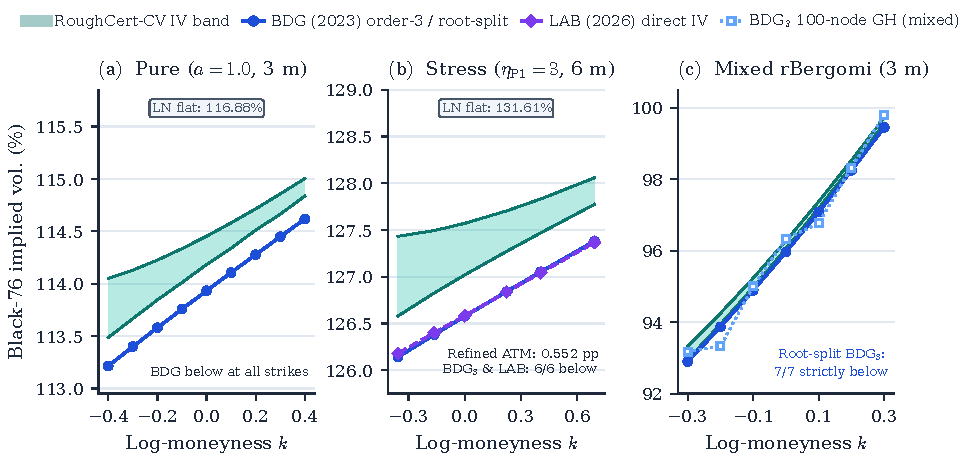
\includegraphics[width=\textwidth]{figures/fig_v3_04_vix_smiles.pdf}}{\fbox{fig\_v3\_04 pending}}
\caption{\RoughCertCV{} Black-76 implied-volatility bands versus BDG~(2023), LAB~(2026), and lognormal
proxies. (a) Pure rBergomi ($a=1.0$, $3$\,m); (b) refined stress cell ($\eta_{\mathrm{P1}}=3$, $6$\,m);
(c) mixed rBergomi ($3$\,m, root-split versus the authors' $100$-node implementation).}\label{fig:vix_smiles}
\end{figure}
\ifTwoColumn\else\FloatBarrier\fi
